
% ════════════════════════════════════════
% 问题分析（2.问题分析.tex）
% ════════════════════════════════════════
\section{问题分析}

本文按"先计划、后兑现"的时间结构逐层展开。问题一在信息完备下求解单日调度，属标准线性规划\cite{yunchouxue2021}：以全天购电费用最小为目标，在储能容量、充放电功率与日循环约束下输出各 10 分钟间隔的购电与充放电功率。问题二推广为"预测—决策—结算"的全年逐日滚动优化：每天 0:00 按历史预测残差构造 9 个情景建立两阶段随机线性规划\cite{birge2011}，实际功率到达后按供电缺口以 5 倍电价结算紧急购电、富余电量计为弃电，日末储电量传递至次日；1 月为预热期，费用汇总仅统计 2 月 1 日—12 月 31 日。问题三引入 0:00、6:00、12:00、18:00 四个时刻的光伏滚动预报\cite{liuweiliang2018}，以分段惩罚刻画计划调整并用上境变量线性化。问题四将电价逐间隔替换为实时波动电价，重算问题二与问题三。四问的流程与衔接如图~\ref{fig:overall_analysis}~所示。

\begin{figure}[H]
    \begin{center}
        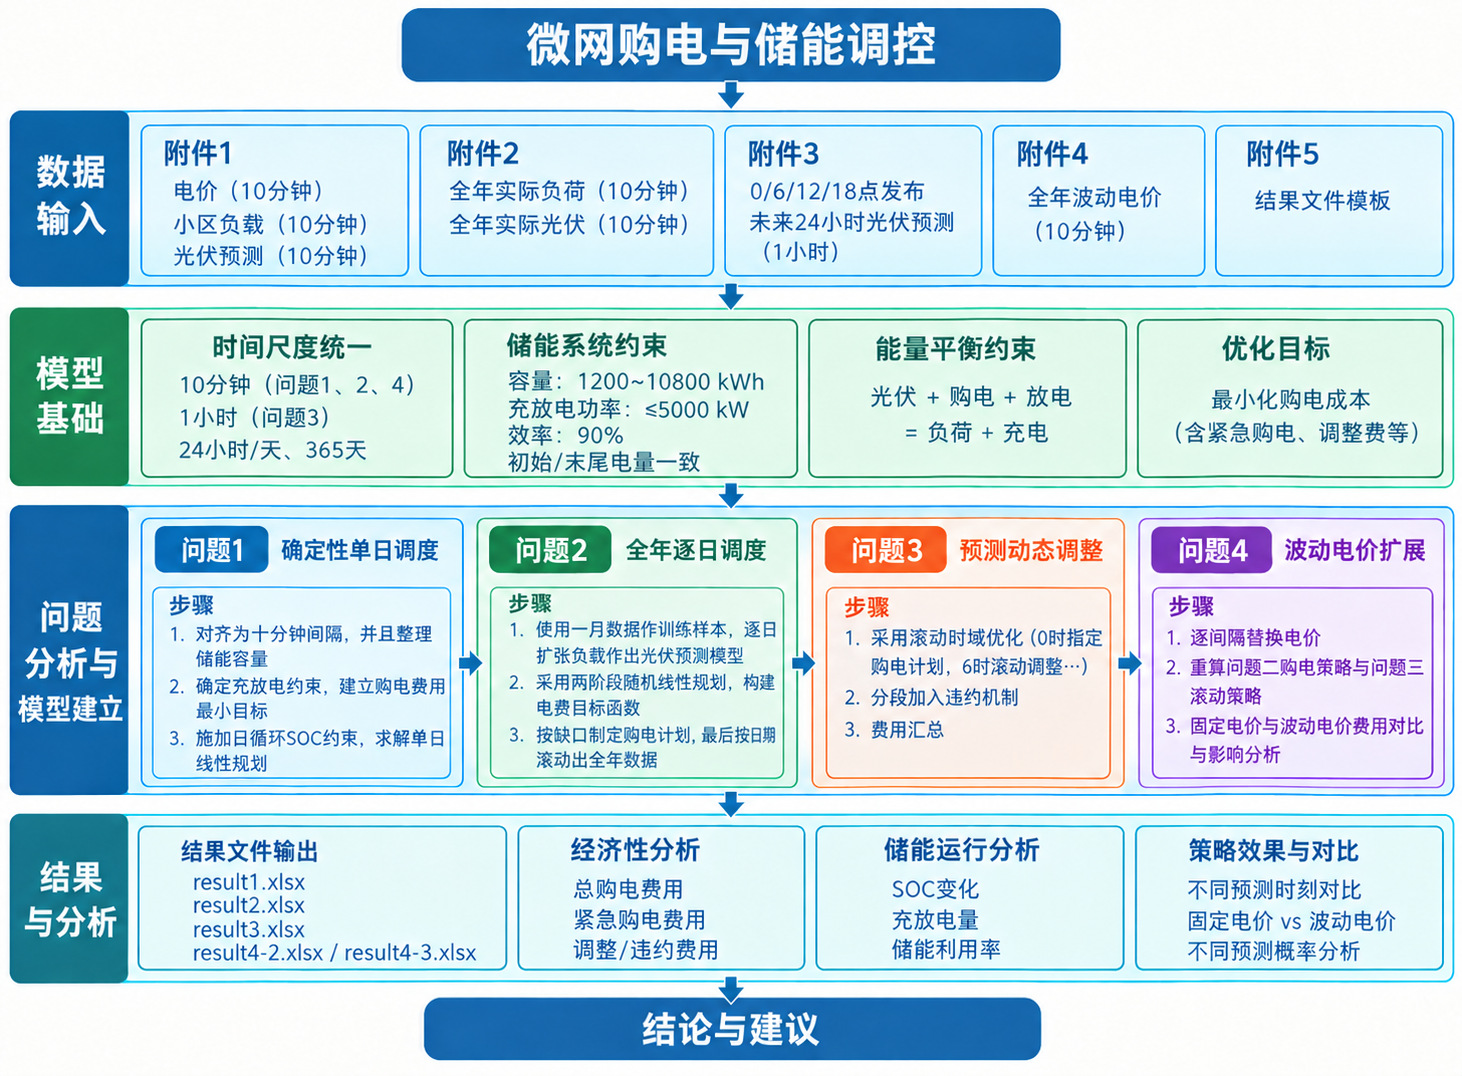
\includegraphics[width=0.96\textwidth]{支撑材料/pic/图1_问题分析总体流程图.png}
        \caption{问题分析总体流程图}
        \label{fig:overall_analysis}
    \end{center}
\end{figure}
